\begin{example}
Περιγράψτε το μετασχηματισμό που περιστρέφει ένα δοσμένο σημείο $Q(x, y)$ κατά γωνία $\theta$ ως προς ένα δοσμένο κέντρο περιστροφής $P(h, k)$ (σχήμα 3.10). Υπολογίστε το σχετικό πίνακα $R_{\theta, P}$ που θα εκτελεί το συγκεκριμένο μετασχηματισμό.

\end{example}

\begin{solution}
	


Εφαρμόζουμε γεωμετρικούς μετασχηματισμούς. Θα προσπαθήσουμε να αναγούμε το ζητούμενο μετασχηματισμό σε σύνθεση βασικών μετασχηματισμών. Εκτελούμε τα ακόλουθα βήματα:

Βήμα 1: Μεταφέρουμε το κέντρο περιστροφής $P$ στην αρχή των αξόνων. Η μεταφορά θα γίνει κατά διάνυσμα $V$ όπου $V = -h\hat{i} - k\hat{j}$, όπου $\hat{i}, \hat{j}$ τα μοναδιαία διανύσματα στους άξονες $x$ και $y$ αντίστοιχα (Σχήμα 3.11).

\[
\text{Βασικός πίνακας μετασχηματισμού: } T_v
\]



Βήμα 2: Εκτελούμε περιστροφή κατά γωνία $\theta$ ως προς την αρχή των αξόνων εφαρμόζοντας το μετασχηματισμό $R_\theta$ (Σχήμα 3.12).

\[
\text{Βασικός πίνακας μετασχηματισμού: } R_\theta
\]



Ο ζητούμενος μετασχηματισμός προκύπτει ως σύνθεση των παραπάνω:

\[
R_{\theta,P} = T_{-V} \circ R_\theta \circ T_V
\]

\begin{figure}[h!]
	\begin{center}
		\begin{minipage}[b]{0.48\textwidth} % Top-left image
		%    \centering
		    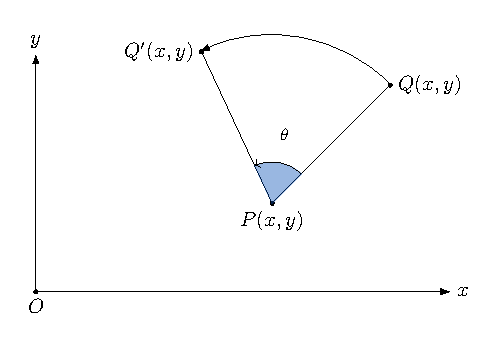
\includegraphics[scale=1]{Chapter2/figure10.pdf}
		    \captionof{figure}{Βήμα 1}
		\end{minipage}%
	\hfill
		\begin{minipage}[b]{0.48\textwidth} % Top-right image
		%    \centering
			    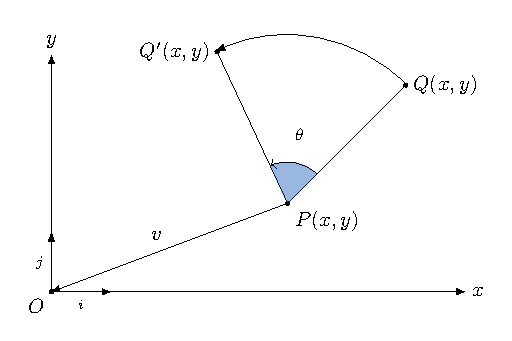
\includegraphics[scale=1]{Chapter2/figure11.pdf}
		    \captionof{figure}{Βήμα 2}
		\end{minipage}
	\end{center}
\end{figure}


\begin{figure}[h!]
	\begin{center}
		\begin{minipage}[b]{0.48\textwidth} % Top-left image
		%    \centering
		    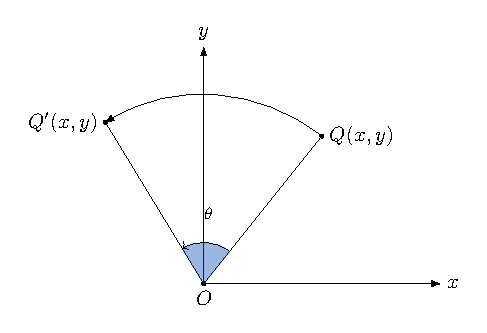
\includegraphics[scale=1]{Chapter2/figure12.pdf}
		    \captionof{figure}{Βήμα 3}
		\end{minipage}%
	\hfill
		\begin{minipage}[b]{0.48\textwidth} % Top-right image
		%    \centering
			    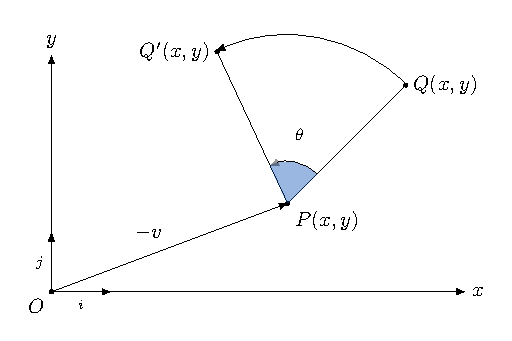
\includegraphics[scale=1]{Chapter2/figure13.pdf}
		    \captionof{figure}{Βήμα 4}
		\end{minipage}
	\end{center}
	\caption{Περιστροφή σημείου $Q(x,y)$ κατά γωνία $\theta$ ως προς ένα δοσμένο κέντρο περιστροφής $P(h,k)$}
\end{figure}

Εφαρμόζοντας τους βασικούς γνωστούς πίνακες προκύπτει ότι:

\[
R_{\theta,P} =
\begin{bmatrix}
1 & 0 & 0 \\
0 & 1 & 0 \\
-h & -k & 1
\end{bmatrix}
\cdot
\begin{bmatrix}
\cos\theta & -\sin\theta & 0 \\
\sin\theta & \cos\theta & 0 \\
0 & 0 & 1
\end{bmatrix}
\cdot
\begin{bmatrix}
1 & 0 & 0 \\
0 & 1 & 0 \\
h & k & 1
\end{bmatrix}
=
\begin{bmatrix}
\cos\theta & -\sin\theta & -h\cos\theta + k\sin\theta + h \\
\sin\theta & \cos\theta & -h\sin\theta - k\cos\theta + k \\
0 & 0 & 1
\end{bmatrix}
\]

Οι συντεταγμένες του καινούργιου σημείου $Q'(x', y')$ προκύπτουν από την επίδραση του $R_{\theta,P}$ πάνω στο αρχικό σημείο $Q(x, y)$:

\[
\text{Τελικά:}
\begin{bmatrix}
x' \\ y' \\ 1
\end{bmatrix}
=
R_{\theta,P}
\begin{bmatrix}
x \\ y \\ 1
\end{bmatrix}
\]
\end{solution}